\chapter{Introduzione}
\section{Massimi e minimi}
\begin{enumerate}
\item \underline{\underline{Max e min assoto}} \textrightarrow \underline{\underline{relativi}} prendendo come esempio la funzione $\sin$
  \begin{center}
    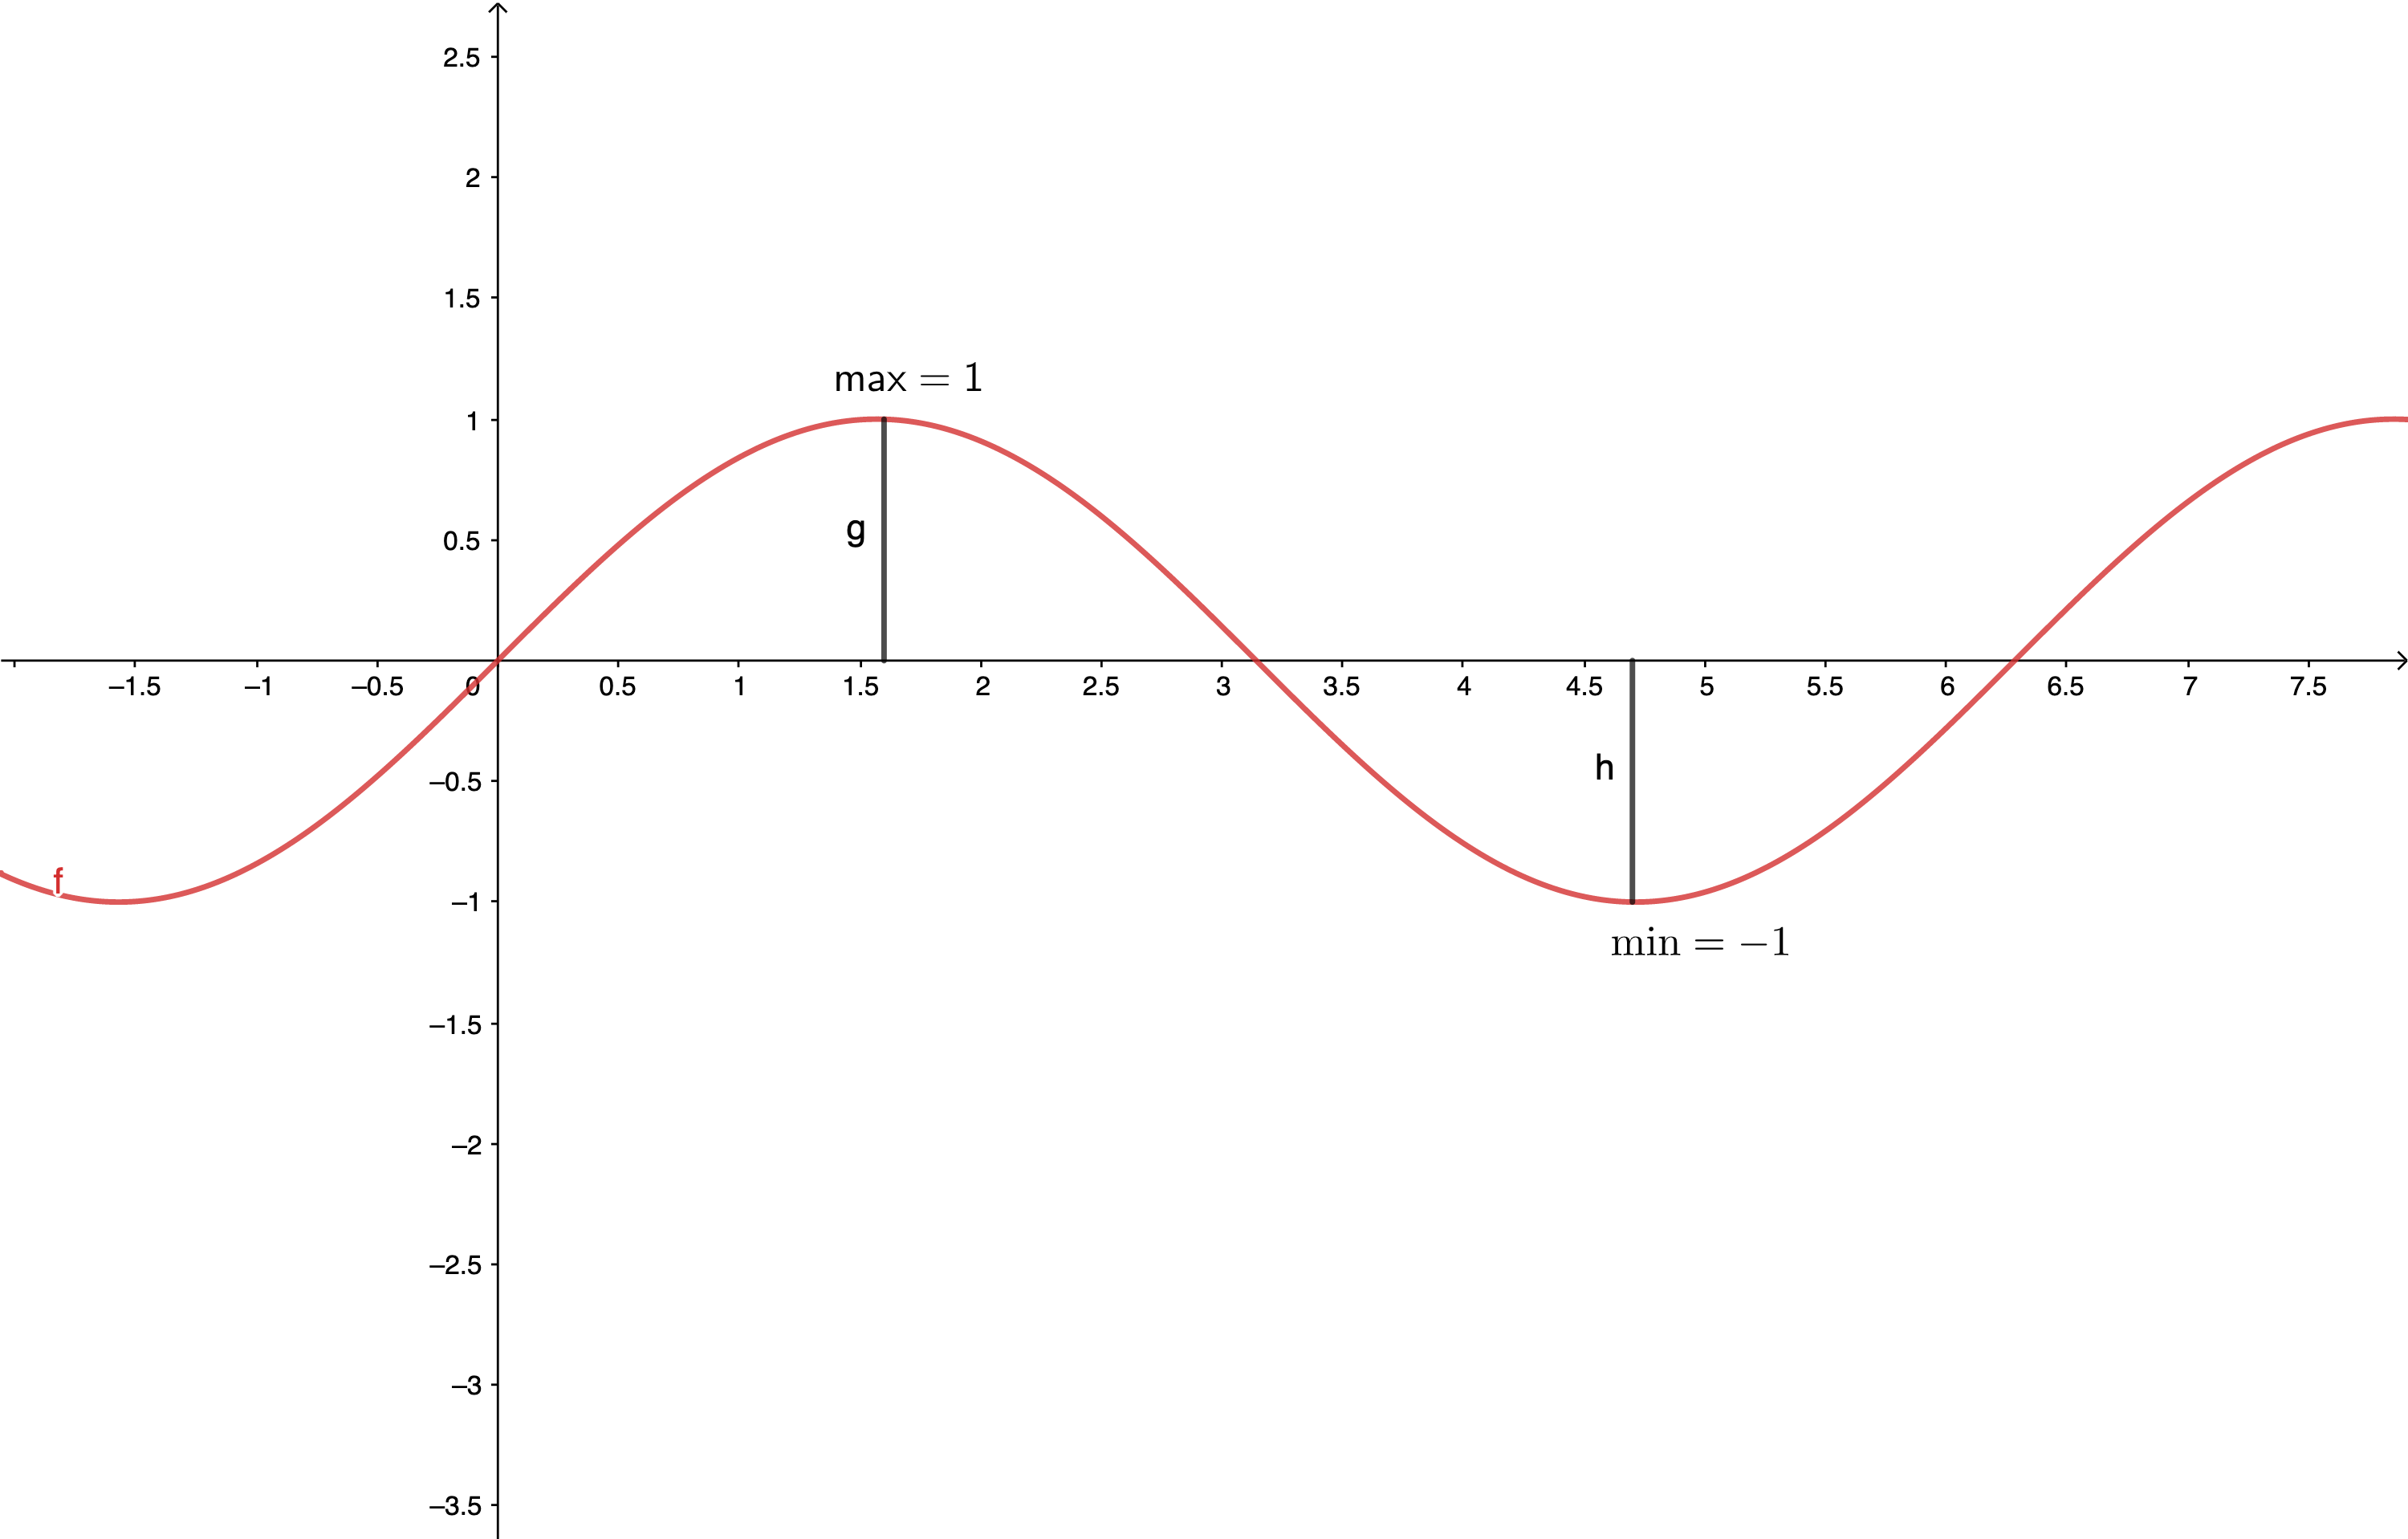
\includegraphics[width=8cm]{img/sin_ex.png}
  \end{center}
  In questo caso il massimo assoluto e relativo della funzione è 1 e il minimo assoluto e relativo è -1, $\min(|x|)=0$ e $\max (\abs{x})$= (negli estremi frontiera). 
\end{enumerate}
\begin{esempio}
  Prendendo la funzione con due incognite $z=x^2+y^2$ e $z=1$
  \begin{enumerate}
  \item deminio $0\leq z\leq 1$
  \begin{center}
    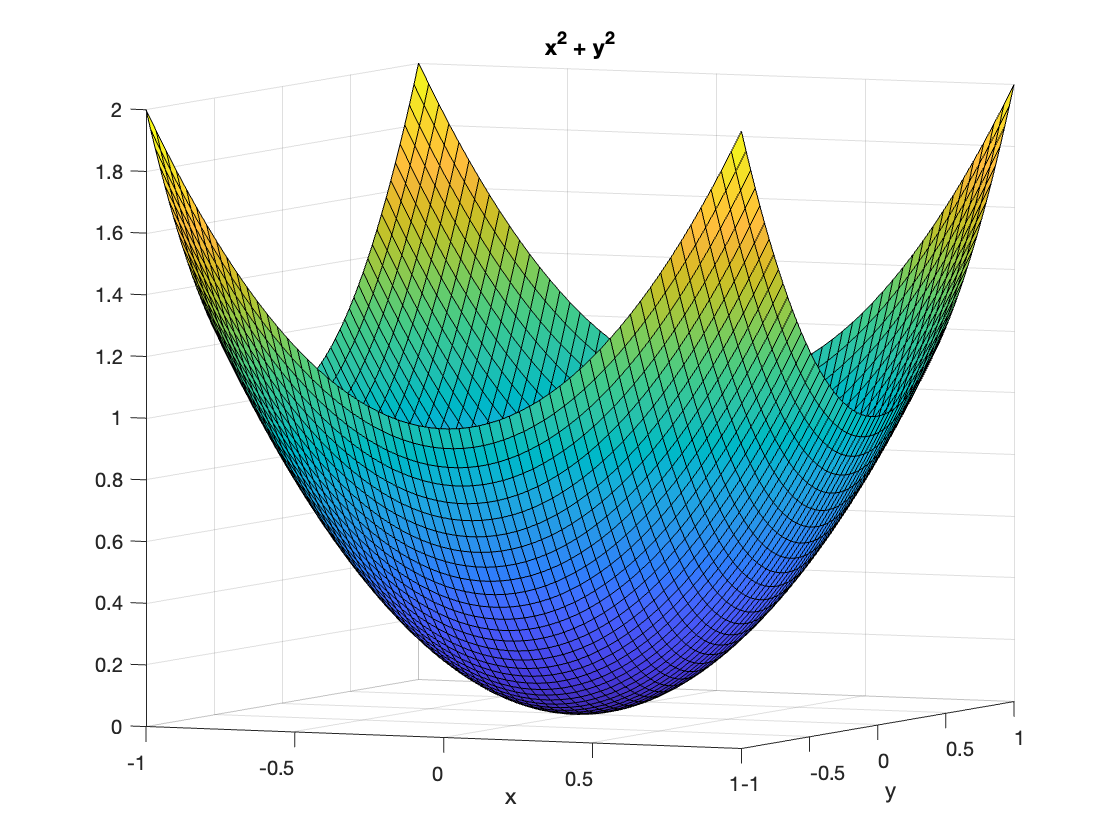
\includegraphics[width=8cm]{img/par.png}
  \end{center}
 
  \end{enumerate}
\end{esempio}
    
\section{limiti}
\begin{defi}
	il limite finito è il limite di f(x,y) per $(x,y)\to (x_0,y_0)$ $(\lim\limits_{(x,y)\to(x_0,y_0)} f(x,y)=L)$ se $\forall\xi >0: \forall (x,y)\in I(x_0,y_o)/\left\{x_0,y_0\right\}$
	\begin{equation*}
		\abs{\underbrace{f(x,y)-L}_{\text{\shortstack{Distanza}}}}<\xi
	\end{equation*}
	se $(x_0,y_0)\xi D(f)$ $(\exists f(x_0,y_0))$
	\begin{equation*}
		\boxed{\lim_{(x,y)\to (x_0,y_0)} f(x,y)\underbrace{f(x,y)-L}_{\text{\shortstack{Continua}}}}
	\end{equation*}
tutti i polinomi sono funzioni continue	
\end{defi}
\begin{esempio}
	\begin{equation*}
		\begin{matrix}
			\lim_{(x,y)\to +\infty}(x^2+y^2)e^{x^2+y^2}
		\end{matrix}
	\end{equation*}
\end{esempio}
\subsection{Teoremi}
\begin{enumerate}
	\item Unicità del limite
	\begin{equation*}
		\abs{l_2-l_1}\leq \abs{}
	\end{equation*}
	\item Teorema del confronto
	\item teorema della permanenza del segno
	\item teorema della composizione delle funzioni continue\footnote{se si vanno a comporre delle funzioni utilizzando due o più funzioni continue si otterrà sempre una funzione continua}
\end{enumerate}
in generale i teoremi sulle operazioni
\begin{esempio}
	Dato $f(x,y)=\begin{cases} x^2+y^2\\ k&(x,y)=(0,0)\end{cases}$
	\begin{equation*}
		\begin{matrix}
			\lim_{(x,y)\to(0,0)}\frac{x^3}{x^2+y^2}=\begin{cases}
				x=\rho \cos y\\
				y=\rho \sin y
			\end{cases}\\
			\lim_{}
		\end{matrix}
	\end{equation*}
	
	
\end{esempio}
\chapter{Esercizi svolti}
\section{Teorema di Gauss e Stokes}
\begin{esercizio}
	Usando il teorema di Stokes, calcolare il flusso del rotore del campo vettoriale \textbf{F:}$\mathds{R}\to \mathds{R}^3$ definito da
	\begin{equation*}
		F(x,y,z)=\left(-x^2y, x^3+z^2,\arctan e^{x+y+s}\right)
	\end{equation*}
	attraverso la superficie
	\begin{equation*}
		\sum:\begin{cases}
			x^2+y^2+z^2=4\\
			z\geq 0
		\end{cases}
	\end{equation*}
	orientata secondo i versori uscenti dall'origine.
\end{esercizio}
\begin{svol}
	Il teorema di Stokes assicura che il flusso $\phi_\Sigma$ (rot $F$) del rotore di $F$ attraverso la calotta
	orientata $\sum$ coincide con il lavoro del campo $F$ lungo il bordo $\Gamma(\sum)$ di $\sum$ orientato
	coerentemente con $\sum$ (cioè secondo il verso di un osservatore che, disposto come il campo normale che
	orienta $\sum$, percorre $\Gamma(\sum)$ vedendo $\sum$ alla sua sinistra)\\
	La superfocoe $\Sigma$ è la semisfera di contro l'origine e raggio 2 contenuta nel semispazio $z\geq 0$ e
	dunque il suo bordo $\Gamma =\Gamma (\Sigma)$ è la circonferenza del piano $xy$ di centro l'origine e raggio 2,
	che ammette la rappresentazione parametrica
	\begin{multicols}{2}
		\begin{equation*}
			\Gamma:
			\begin{cases}
				x=2\cos t\\
				y=2\sin t, & t\in [0,2\pi],\\
				z=0
			\end{cases}
		\end{equation*}
	\end{multicols}
	Tale rappresentazione risulta coerente con l'oriantamento di $\sigma$, in quanto, al crescere di $t$,
	il punto $\gamma= (2\cos t, \sin t, 0)$ si muove lungo $\Gamma$ come in figura. Dunque, poiché
	\begin{equation*}
		F(\gamma(t))=F(2\cos t, 2\sin t,0)=(-8\cos^2t\sin t, 8\cos^3t, \arctan e^{2\cos t+2\sin t}),
		\gamma^\prime (t)=(2\sin t, 2\cos t, 0), 
	\end{equation*}
	si ha
	\begin{equation*}
		\phi(rot F)= \int_\Sigma F*dP=\int^{2x}_0F(\gamma(t)) *\gamma(t)dt=\int (16\cos^2t+16\cos^4t)dt =
		16\int^{2x}_{0}\cos^2tdt=16\left[\frac{t+\cos t \sin t}{2}\right]^{2x}_0=16x.
	\end{equation*}
\end{svol}
\clearpage
\begin{esercizio}
	Calcolare il lavoro del campo vettoriale
	\begin{equation*}
		F(x,y,z)=(\sin(x^2+z)- 2yz, 2xy+\sin(y^2+z),\sin(x^2+y^2))
	\end{equation*}
	lungo la circonferenza
	\begin{equation*}
		\begin{cases}
			x^2+y^2=1\\
			z=3
		\end{cases}
	\end{equation*}
	percorso in modo che la proiezione sul piano $xy$ giri in senso orario (rispetto ad un osservatore disposto come l'asse $z$).\\
\end{esercizio}
\begin{svol}
	Vista l'espressione del campo, il calcolo dipende dal lavoro richiesto non pare agevole. D'altra parte, risulta
	\begin{equation*}
		\begin{matrix}
			rot F= \begin{vmatrix}
				i & j & k\\
				\frac{\partial}{\partial x} & \frac{\partial}{\partial y} &  \frac{\partial}{\partial z}\\
				\sin(x^2+z)-2yz & 2xz+\sin(y^2+z) & \sin (x^2+y^2)
			\end{vmatrix}
		\end{matrix}
	\end{equation*}
	
\end{svol}
\chapter{Derivate parziali}
\begin{defi}
    Sia D un insieme aperto di $R^2$ e $f(x,y)$ definita in D. Consideriamo il punto
    $(x_0,y_0)\subset D$ e un suo interno $D_\delta (x_0,y_0)\subset D.$ Consideriamo il punto
    $(x_0+h,y_0)\in D$, $h\in \mathds{R}$. Costruiamo il rapporto incrementale
    \begin{equation}
        \frac{f(x_0+h,y_0)-f(x_0,y_0)}{h}.
    \end{equation}
    \begin{table}[ht]  
      	\centering
        \begin{tabular}{|l|}
            \hline
            Definizione di Derivata parziale rispetto a x.\\\hline\hline
            Se esiste finito il
            $\lim\limits_{h\to0}\frac{f(x_0+h,y_0)-f(x_0,y_0)}{h}=f_x(x_1,y_0)$,\\
            definiamo la funzione derivabile rispetto a $x$ in $(x_0,y_0)$.\\\hline
        \end{tabular}
    \end{table}
    Si usano anche i simboli
    \begin{equation}
      \begin{matrix}
        \frac{\partial f}{\partial x}(x_0,y_0), & \frac{\partial f}{\partial y}(x_0,y_0).
      \end{matrix}
    \end{equation}
    Si estendono le regole di derivazione sia per le operazioni che per le funzioni elementari e composte.
\end{defi}
\begin{esercizio}
  Calcolare $f_x(4,1)$ con $f(x,y)=\log(x-y^2)$
  \begin{equation*}
    f_x(4,1)=\lim_{h\to0}\frac{\ln(x-1)-\ln3}{h}=\lim_{h\to 0}\frac{\ln\left(1+\frac{h}{3}\right)}{h}
  \end{equation*}
  (si è utilizzato il limite notevole: $\lim\limits_{t\to 0}\frac{\ln(1+t)}{t}=1,$
  {\color{red}(*)}) oppure,
  \begin{equation*}
    f_x(4,1)=\lim_{x\to 4}\frac{\ln(x-1)-\log(3)}{x-4}=\lim_{x\to 4} \frac{1}{3} \frac{\ln\frac{x-1}{3}}{\frac{x-4}{3}}=\lim_{x\to 4}\frac{1}{3}\frac{\ln\left(1+\frac{x-4}{3}\right)}{\frac{1}{3}},
  \end{equation*}
  dove è stato utilizzato il limite notevole {\color{red}(*)}
\end{esercizio}
\section{Significato geometrico della derivata parziale prima}
$\frac{\partial f}{\partial x}(x_0,y_0)$ è il coefficiente angolare della retta tangente al
grafico di $f$ nel punto $P=(x_0, y_0, f(x_0, y_0))$ che giace sul piano $y=y_0,$ analogamente
$\frac{\partial f}{\partial y}(x_0,y_0)$ è il coefficiente angolare della retta tangente al
grafico di $f$ nel punto $P=(x_0, y_0, f(x_0, y_0))$ che giace sul piano $x=x_0$.\\
Indichiamo con $\Delta f=(f_x,f_y)$ che chiamiamo gradiente di $f$, il vettore di componenti le
derivate parziali prime (rispetto alla direzioni degli assi $x$ e $y$). Si demostra che se non è
nullo, il vettore gradiente $\Delta f=(f_x,f_y),$ (con $f$ differenziabile) indica la direzione
di massima pendenza di $f$.
\begin{esempio}
  Se consideri la funzione
  \begin{equation*}
    \begin{matrix}
      f(x,y)=x+2y, & (x,y)\in R^2
    \end{matrix}
  \end{equation*}
  si ottiene:
   \begin{equation*}
    \begin{matrix}
      f_x=1 & f_y=2, & \text{costante su } \mathds{R}\\
      & \nabla f = (1,2),
    \end{matrix}
  \end{equation*}
  ed seprime la direzione e il verso nel piano di base $x,y$ in cui conviene muoversi per
  ottenere il massimo incremento della funzione $f$ (a parità di percirsi nel piano $x,y$).
\end{esempio}



